\documentclass{mprop}
\usepackage{graphicx}
\usepackage[colorinlistoftodos]{todonotes}

% alternative font if you prefer
% comment this out to go back
\usepackage{times}

% for alternative page numbering use the following package
% and see documentation for commands
%\usepackage{fancyheadings}


% other potentially useful packages
%\uspackage{amssymb,amsmath}
%\usepackage{fancyvrb}
%\usepackage[final]{pdfpages}
\usepackage{enumerate}
\usepackage{enumitem}
\usepackage[colorlinks=true, allcolors=blue]{hyperref}
\usepackage[colorinlistoftodos]{todonotes}
\usepackage{listings}
\usepackage[newfloat]{minted}
\usemintedstyle{emacs}
\usepackage{pgfplots}
\usepackage{enumerate}
\usepackage{enumitem}
\usepackage{url}
\usepackage{amssymb}
\usepackage{amsmath}
\usepackage{caption}
\usepackage{adjustbox}
\usepackage{subcaption}
\usepackage{inconsolata}
\usepackage{graphics}
\pgfplotsset{compat=1.8}
\usepackage{tabu}
\usepackage{multirow}
\newcommand{\code}[1]{\texttt{#1}}
\newenvironment{codelisting}{\captionsetup{type=listing}}{}
\SetupFloatingEnvironment{listing}{name=Code Sample}

% Use “\cite{NEEDED}” to get Wikipedia-style “citation needed” in document
\usepackage{ifthen}
\let\oldcite=\cite
\renewcommand\cite[1]{\ifthenelse{\equal{#1}{NEEDED}}{\ensuremath{^\texttt{[citation~needed]}}}{\oldcite{#1}}}

\usepackage{xcolor,colortbl}
% A package which allows simple repetition counts, and some useful commands
\usepackage{forloop}
\newcounter{loopcntr}
\newcommand{\rpt}[2][1]{%
  \forloop{loopcntr}{0}{\value{loopcntr}<#1}{#2}%
}
\newcommand{\on}[1][1]{
  \forloop{loopcntr}{0}{\value{loopcntr}<#1}{&\cellcolor{gray}}
}
\newcommand{\onx}[1][1]{
  \forloop{loopcntr}{0}{\value{loopcntr}<#1}{&\cellcolor{orange}}
}
\newcommand{\off}[1][1]{
  \forloop{loopcntr}{0}{\value{loopcntr}<#1}{&}
}

\definecolor{orange}{HTML}{FF7F00}

\renewcommand{\arraystretch}{1.5}

\begin{filecontents*}{data.csv}
name map length time
allterms 	0.4554	358.5  	2.51435
ne 			0.3979  93.45  	0.4132
tfidf 		0.3038  10  	0.13675
subject 	0.184  	9.75  	0.1578
\end{filecontents*}

\begin{document}

%%%%%%%%%%%%%%%%%%%%%%%%%%%%%%%%%%%%%%%%%%%%%%%%%%%%%%%%%%%%%%%%%%%
\title{Research Proposal: Smart Sensitivity Review}
\author{Kelvin Fowler}
\date{\today}
\maketitle
%%%%%%%%%%%%%%%%%%%%%%%%%%%%%%%%%%%%%%%%%%%%%%%%%%%%%%%%%%%%%%%%%%%

%%%%%%%%%%%%%%%%%%%%%%%%%%%%%%%%%%%%%%%%%%%%%%%%%%%%%%%%%%%%%%%%%%%
\tableofcontents
\newpage
%%%%%%%%%%%%%%%%%%%%%%%%%%%%%%%%%%%%%%%%%%%%%%%%%%%%%%%%%%%%%%%%%%%

%%%%%%%%%%%%%%%%%%%%%%%%%%%%%%%%%%%%%%%%%%%%%%%%%%%%%%%%%%%%%%%%%%%
\section{Introduction}\label{intro}
The National Archives are subject to the Freedom of Information Act (2000)~\footnote{http://www.legislation.gov.uk/ukpga/2000/36/contents}. 
This means that they must respond to freedom of information requests and release documents after a certain amount of time.
There are many reasons why a document may be withheld~\footnote{https://ico.org.uk/for-organisations/guide-to-freedom-of-information/refusing-a-request/} \footnote{http://www.legislation.gov.uk/ukpga/2000/36/part/II}, especially if the document is deemed to contain sensitivities.
For example, a document may contain the name of confidential informants whose lives would be in danger if the document were released to the public.
For this reason there is a rigorous review process in place at The National Archives. Archivists must review documents and decide if they contain sensitivities.
One aspect of this review process is the comparison of document contents to information in the public domain, such as news articles.
If there is potentially sensitive information within a document, but the information is already known to the public, then the document can be released without cause for concern.
This is not a trivial task and it currently requires the archivists to use public search engines to query the public domain.
Not only is this slow, it is insecure and releases potentially sensitive information to an external service.
Further, with the recent mass adoption of digital documents, more documents must be kept than ever before with every email and digital document being automatically archived.
The sensitivity review process is struggling to keep up with the rate of document generation~\cite{allan2014record} and there is an increasing burden on archive facilities to decide ``what to keep''~\cite{moss2012have} as the collections of documents grow in size each day.

This abundance of digital documents presents an opportunity to adjust the sensitivity review process and introduce assistive technology to make the process easier.
Generally, this type of classification task falls into the domain of Information Retrieval (IR), which is the process of providing information relevant to a given information need.
Some work has been done to apply IR in the automatic classification of documents as sensitive (see Section~\ref{background_survey.sensitivity_review}), however this proposal seeks to address the identification of public domain knowledge task described above.
The information need is public domain documents relating to the contents of a given document which is to be reviewed.
If these public domain documents (such as news articles) can be automatically presented to the reviewer alongside the document for review, this would significantly decrease the workload and security concerns attached to this part of the process.
We do not seek to outright replace the role of manual review with technology, and it has been noted in the past that archivists are reluctant to trust technology alone in the sensitivity review process~\cite{gollins2014using}.

This task of identifying public domain knowledge in relation to the contents of potentially sensitive documents has already been tackled in part by a Level 4 Project at the University of Glasgow. 
The system generated queries automatically from documents which were potentially sensitive and ran them through an IR search engine to return relevant public domain documents.
The system also provided a prototype user interface for presenting the results to manual reviewers.
The system proved successful, though the process of generating queries from potentially sensitive documents did not extend far beyond the extraction of named entities. 
These source documents contain other information which can be automatically extracted and included in a query.
This proposed research seeks to expand upon the system created last year in order to improve it's effectiveness and provide better public domain results for any given potentially sensitive document.
Some potential avenues for this expansion were identified during the evaluation stage of the L4 Project, such as extraction of temporal information and the use of machine learning.
We propose to use these techniques, and others, to generate further queries from potentially sensitive documents.
Further, we wish to investigate improvements to the entire retrieval system, in addition to the query generation phase.

\subsection{Terminology}
From henceforth a potentially sensitive document from which queries are generated will be called a \textbf{Source Document}.
In some cases, documents will be used which are not potentially sensitive, but are representative of the types of documents encountered during  sensitivity review.
A public domain document which is to be retrieved by the search engine will be called a \textbf{Target Document}.
Target Documents will be public domain documents such as news or Wikipedia articles.

Analogously, the set of all Source Documents will be referred to as the \textbf{Source Collection} and a set of Target Documents will be referred to as a \textbf{Target Collection}.
Potentially, the collection of all target documents is enormous, and consists of every public domain document. We will deal with some specific limited subsets of target documents.

The project which was completed last year will be referred to as the \textbf{L4 Project}.

\subsection{Structure}
This research proposal will take the following structure. 
In Section~\ref{problem_statement} we will more formally define the problem this research seeks to address, and how this research will contribute to the field of IR. 
In Section~\ref{background_survey} related literature is reviewed in order to investigate the proposed projects relevance and prompt discussion of potential avenues for this research to take. 
Section~\ref{proposed_approach} outlines the proposed approach the research will take, as well as detailing some preliminary investigations into the feasibility of these goals. 
This includes some discussion of motivations for choices of technologies.
Finally, Section~\ref{work_plan} highlights some proposed implementation details, deliverables and potential dates for their completion.

%%%%%%%%%%%%%%%%%%%%%%%%%%%%%%%%%%%%%%%%%%%%%%%%%%%%%%%%%%%%%%%%%%%
\section{Statement of Problem}\label{problem_statement}
With some motivation in mind for the problem this proposed research will address, we must now consider how to formalize our aims. 
As will be discussed in more detail in Section~\ref{background_survey.previous_project} the L4 Project began by investigating the use of named entities present in source and target documents.
Named Entities are words or phrases (generally proper nouns) referring specifically to people, places or organisations.
These named entities were identified in both source and target documents so that they could be directly matched during retrieval. 
Time dictated that the approaches did not extend far beyond this, however the findings provided useful insights which have been used to formulate some of the ideas in this proposal. 
Some other extractable items in addition to named entities are present in the bodies of source documents such as dates, subjects, noun phrases, verb phrases and other n-grams. 
Generally, there exists reasonable methods for automatic extraction of many of these such as the Stanford NLP Tool-kit~\cite{manning2014stanford}. 
Further, the specification for the L4 Project originally mentioned making use of some machine learning techniques. 
This was not investigated due to time constraints, but machine learning (especially learning to rank) has been shown to improve performance in many retrieval tasks (see Section~\ref{background_survey.l2r}).
These methods will be explored in detail throughout Sections~\ref{background_survey}~and~\ref{proposed_approach}. 
We wish to combine these ideas to create a performant retrieval system which can return target documents which are relevant to the content of a source document, in a way which is assistive to sensitivity review. 
%We wish to make use of relevant IR technologies outside of the previously explored query generation through named entity extraction and to discover what information a source document contains that is the most important for the task of retrieval of public domain knowledge.
Relevant IR technologies can be employed to extend upon the extraction of named entities, allowing us to formulate queries containing other sources of information.

\subsection{Research Questions}
The following research questions formalize the above discussion and describe the goals of this proposed project.
\begin{enumerate}[label=\textbf{RQ.\arabic*}]
\item \textit{What extractable information within the body of source documents (such as named entities, temporal References and other n-grams) are most important in the formation of a query for retrieval of public domain documents relevant to events and concepts mentioned in a source document? }

\textbf{RQ1} has already been tackled in part. 
The L4 Project showed that named entities extracted from source documents provide a good base query with which to perform retrieval. 
However it was also identified that by removing much of the other information and context from the source document we lost some search accuracy (see Section~\ref{background_survey.previous_project} for more detail). 
The task of comparison of public domain information in sensitivity review often deals with references to specific events. 
These events occur at a given time and so the temporal information present in source documents can be used to identify these time frames. 
We must also discover what other information contained in source documents can be leveraged to assist this task.
Context surrounding named and temporal entities could be important. 
The challenge remains to identify what constitutes context and how it can be leveraged.

\item \textit{Can a comprehensive retrieval model be produced to generate queries from unseen source documents to retrieve public domain documents related to events and notions inside the source document?}

\textbf{RQ2} addresses a potentially more difficult question. 
In \textbf{RQ1} we discuss the extraction of features from source documents such as temporal entities and named entities. 
We must form these extracted features in to a query and run it through some IR search engine. 
We must therefore create a supporting framework which allows for the seamless extraction of these features and the ability to use them in queries. 
Not only that, there is much more to IR than sound query formulation. 
Machine learning techniques such as learning to rank and query expansion techniques like pseudo-relevance feedback can be applied to improve performance. 
We must consider which techniques are most appropriate in the scenario of retrieval of public domain knowledge and effectively apply and integrate them. 
This entire system must be empirically evaluated in order to answer \textbf{RQ2}.
\end{enumerate}

These research questions allow us freedom to investigate multiple avenues of query generation and retrieval techniques. In Section~\ref{proposed_approach.evaluation} we give more detailed hypotheses, relating to these research questions, upon which to evaluate our proposed work.

\subsection{Scope of this Project}
We now define the expected scope of this proposed project. 
Specifically, we define what we propose to address, what we may address if time permits and what we will not investigate at all.
Clearly, we must investigate, implement and evaluate a system which can answer the above research questions (\textbf{RQ1} \& \textbf{RQ2}). 
In order to do this, we must create a system which generates queries from documents, runs these queries against a target collection and analyses the quality of the results.

Assuming this initial research is done in satisfactory time, other avenues may be explored such as knowledge base linking and query expansion. 
More detail on these concepts can be found in Section~\ref{background_survey}.

This proposed project will explicitly not focus on developing or improving any kind of user interface. 
This was a sizeable aspect of the L4 Project, however will not be in the scope of this proposed work.

\subsection{Contributions}
This research will contribute an improvement to the understanding of the formation of queries from documents. 
As far as we know, it will be the first work of its kind which seeks to combine the ideas of named entity extraction, temporal entity extraction and learning to rank in order to assist sensitivity review.
Specific techniques for query generation from documents will be described and empirically evaluated. 
This research has applications in many areas of IR outside of sensitivity review, for example, finding related web pages, news stories or other automatic recommendations.

%%%%%%%%%%%%%%%%%%%%%%%%%%%%%%%%%%%%%%%%%%%%%%%%% BACKGROUND SURVEY/ LIT REVIEW
\section{Background Survey} \label{background_survey}
This section will present an overview of the various pieces of related literature to this proposed research. 
We will discuss previous work completed in the field of sensitivity review as well as other IR studies which are applicable and relevant.

\subsection{Previous Project} \label{background_survey.previous_project}
This proposed project is hinged on the existence of the work completed last year as part of the L4 Project \cite{DissertationKelvinFowler}. 
The L4 Project was very much an investigatory project into the domain of using IR to assist sensitivity review. 
Although the L4 Project focussed heavily on a user interface (work which will not continue in this proposed research) it also began to tackle the task of effective retrieval of target documents given some source document. 
The source document was used to generate a query which could be performed in the IR search engine Terrier, against the collection of target documents.
Retrieval using these generated queries was empirically evaluated in order to understand the performance of different query formulations. 
The evaluation results of the L4 Project form a baseline of performance that we wish to improve upon in this proposed research.
They also provide good indication of which avenues to proceed or ignore.

The implementation of the L4 Project can also be reused as a starting point for this proposed research. 
It features some custom indexing tokenizers which extract named entities from source documents. 
This can be expanded to extract the other information we are interested in (temporal entities and other chunks). 
This indexing step allows us to iterate through terms in a document, analyse them and store them in some way. 
The indexing step can be run on source and target documents alike in order to extract and tag the matching information in each.

After indexing the source documents and identifying the named entities, four queries were generated for use in retrieval. These were:
\begin{itemize}
  \item \textit{All Terms Query} - All terms, except stop words, were kept for this query. 
  \item \textit{Named Entities Query} - This query consisted of all the named entities in the document and nothing else. This meant the query was fairly short, however it did not contain any additional context. Named entities were extracted using Stanford Core NLP~\cite{manning2014stanford}. 
  \item \textit{Tf-Idf Named Entities Query} - The named entities were given a Tf-Idf ranking and the top ten were used a query. Tf-Idf is a commonly used IR technique which attempts to estimate term importance through measures of how frequently the term appears in a document compared to a collection of documents.
  \item \textit{Subject Query} - The subject line from a source document was used as a query after having its named entities identified. This was an attempt to add context to the queries, as well as being short and easy to compute.
\end{itemize}

\subsubsection{Evaluation and Findings}
In order to evaluate the system, a test collection was formulated using a sample of source documents. 
These were Wikileaks files which were identified by National Archive's reviewers to be representative of real documents which must be reviewed for sensitivities.
The target collection was a collection of Associated Press news articles.
In order to generate an effective test collection, 20 source documents were chosen and the 4 above queries were generated and run from each. 
The top 20 returned documents for each of these queries was then judged as relevant or non-relevant. 
This formed the test collection.
This was expensive to produce, and so we opt for a different method in this proposed research (see Section~\ref{proposed_approach.evaluation} for details).
These relevance judgements were then used to compute results on the effectiveness of the various query formulations.
It was found that the performance of the \textit{All Terms Query} was the objectively the best, but the query took far too long to perform. 
The query processing time is a measure we must take into account in this proposed project as having an excellent performing query is pointless if it cannot be performed in a reasonable time, especially in the context of assistive review. The shorter \textit{Named Entities Query } was therefore chosen as the most effective considering all factors. Results can be seen in Table~\ref{standard_results}. Figure~\ref{mapgraphs} also shows the clear correlation between query length and processing time, as well as illustrating the point that a significantly shorter (and therefore faster) query can perform reasonably well.

\begin{center}
\begin{table}[h]
\centering
\resizebox{\columnwidth}{!}{%
\begin{tabular}{|c|c|c|c|c|c|}
\hline
Query					& MAP 				& Mean Query  		& Mean Query 			& Mean Reciprocal 		& Mean Precision 	\\ 
						& 					& Length (Words) 	& Processing Time (s) 	& Rank 					& at 4				\\	\hline
All Terms             	& \textbf{0.4554} 	& 358.5             & 2.51435               & \textbf{0.8500}       & \textbf{0.6750} 	\\	\hline
Named Entities 			& 0.3979 			& 93.45    			& 0.4132 				& 0.7526				& 0.5875 			\\	\hline
Tf-Idf Named Entities 	& 0.3038 			& 10                & \textbf{0.13675}      & 0.7236       			& 0.4375 			\\	\hline
Subject               	& 0.1840 			& \textbf{9.75}     & 0.1578                & 0.3367       			& 0.2500 			\\	\hline
\end{tabular}%
}
\caption{Results of Offline Evaluation, Adapted from Level 4 Project~\protect\cite{DissertationKelvinFowler}}
\label{standard_results}
\end{table}
\end{center}

\begin{figure}[H]
\centering
\begin{subfigure}[t]{.5\textwidth}
\centering
\begin{tikzpicture}
 \begin{axis}[
 	ylabel=$MAP$,
    xlabel={Mean Query Processing Time},
    width=0.95\linewidth,
    height=0.5\linewidth
    ]
        \addplot table[x=time,y=map] {data.csv};
    \end{axis}
\end{tikzpicture}
\end{subfigure}%
~
\begin{subfigure}[t]{.5\textwidth}
\centering
\begin{tikzpicture}
 \begin{axis}[
 	ylabel=$MAP$,
    xlabel={Mean Query Length},
    width=0.95\linewidth,
    height=0.5\linewidth
    ]
        \addplot table[x=length,y=map] {data.csv};
    \end{axis}
\end{tikzpicture}
\end{subfigure}
\caption{Analysis of Mean Average Precision (MAP) Scores against Query Processing Time and Query Length. Adapted from Level 4 Project~\protect\cite{DissertationKelvinFowler}} \label{mapgraphs}
\end{figure}

Other noteworthy findings include the fact that Named Entities of the Person type seem to have the biggest bearing on retrieval performance of the 3 named entity types used. 
Also, the extra context present in the \textit{All Terms Query} clearly helped its performance. 
A key takeaway for this research is the challenge of how best to optimize performance while including enough context around named entities. Some qualitative investigation of the performance of certain queries yielded some additional insights. 
Inclusion of temporal data is a potential way to add context to queries.
Further, it was noted that the L4 Project did not make use of the popular process of learning to rank, which is almost ubiquitous in IR systems presently. 
These are both aspects which we propose to work on in the current proposed project.

\subsection{Sensitivity Review} \label{background_survey.sensitivity_review}
Assistive digital sensitivity review is an open challenge in information retrieval, and is being actively tackled, mainly by a team here at The University of Glasgow. 
Together with Timothy Gollins at The National Archives researchers at The University of Glasgow identified the open challenges in the application of IR to sensitivity review~\cite{gollins2014using}.
Most of the work in this topic has been in the realm of automatically classifying sensitivities in documents.
McDonald et al~\cite{mcdonald2014towards} experiment with creating an automatic classification system for sensitivity review. This system uses features such as mentions of foreign countries and subjective sentiment in order to classify sensitivities relating to international relations.
In another investigation McDonald et al~\cite{mcdonald2015using} attempted to identify which parts of speech patterns most likely contained sensitivities relating to content supplied ``in confidence''.
More recently, McDonald et al~\cite{mcdonald2017enhancing} apply machine learning techniques (specifically semantic relationship recognition through word embeddings) to further assist the sensitivity classification process. 

Outside of the work conducted here at the University of Glasgow, Sanchez et al~\cite{sanchez2012detecting} discuss automatically identifying sensitivities in documents in order to sanitize these documents before release. 
They aim to remove personal information by inspecting noun phrases which contain more information than others. 
This is relevant to the work proposed here as the ability to recognise the most informative noun phrases could be used in order to formulate a highly effective query, by disregarding unhelpful terms and phrases.

These sensitivity review papers do not refer to the challenge of public domain knowledge comparison in sensitivity review, but instead tackle other challenges.
While providing good background into the problem domain, they do not necessarily provide information on the specific task we propose. 
This proposed research does not seek to directly classify documents as sensitive or not sensitive, but rather provide a system which can assist manual sensitivity review. 


\subsection{Technology Assisted Review} \label{background_survey.tech_assisted_review}
More generally, sensitivity review falls into the category of Technology Assisted Review (TAR). 
TAR is technology which attempts to improve or assist a manual review process, such as sensitivity review, however some manual aspect must remain.
Other applications of technology assisted review are E-Discovery as described in this overview by Oard and Webber~\cite{oard2013information}, where the retrieval task is retrieving all relevant documents relating to the opposing party in a civil litigation case.
Grossman and Cormack~\cite{cormack2014evaluation} have pushed the capabilities of TAR in E-Discovery through investigation of various machine learning techniques. 
They focus on the application of continuous active learning. This is relevant to this proposed research as it involves a manual reviewer continuously examining suggestions made by the system. 
Interestingly, these manual reviews are added to the training set to further improve the retrieval of yet more documents. 
Not all techniques applicable to E-Discovery are relevant to this proposed research. E-Discovery is a high recall task, in that it is desirable to retrieve \textit{all} relevant documents for a given case. 
This research seeks a high precision retrieval scenario in that we want more relevant documents at higher ranks of the retrieval results.
This type of technology assisted review has also made headlines in recent years when the FBI used technology to assist their review of documents during the 2015 Hillary Clinton email controversy~\cite{cnnclinton}.


\subsection{Temporal Information Retrieval} \label{background_survey.temporal_ir}
Some work has been done in the field of incorporating temporal data into IR systems. 
In Section~\ref{proposed_approach.temporal} we discuss some ways in which temporal information could be applied to this proposed research.
In order to deal with temporal expressions in documents at all, we require a solid foundation to extract and normalize these expressions. Noteworthy temporal taggers include GUTime~\cite{mani2004recent} and more recently SUTime~\cite{chang2012sutime} and Heideltime~\cite{strotgen2010heideltime}. All of these taggers resolve temporal information in documents to the TimeML~\cite{pustejovsky2003timeml} TIMEX3 mark-up language, which defines a specific syntax for defining dates and times. This kind of temporal tagging technology is vital for any kind of use of temporal information from within documents.

In terms of actual applications of temporal information in IR, most relevant to this proposed research is the work of Berberich et al~\cite{berberich2010language} which deals specifically with temporal expressions in queries. 
Beyond basic matching of temporal information as text, Berberich et al~\cite{berberich2010language} use a language modelling approach to attempt to predict the likelihood of temporal expressions in a query being produced from a language model of a given document. Indeed, this begins to answer some of the open questions posed in a review of temporal information in IR~\cite{alonso2011temporal}.
Str{\"o}tgen et al~\cite{strotgen2012identification} describe a method of identifying top relevant temporal expressions in documents. 
That is, identification of which temporal expressions are of most import in a document. 
One can also check which temporal expressions are of most import in relation to a given query (or corpus). 
This has clear applications to this research in two ways. The first being the ability to rank temporal expressions for the purpose of query generation. 
The second being query based features which can be used to retrieve relevant documents (those with more relevant temporal expressions are potentially more relevant).
Li and Croft display in~\cite{li2003time} a ``time based language model'' which promotes in search results documents from a given time period. This has the application in this proposed research of the ability to promote target documents which are from a similar period to the source document.
Jatowt et al~\cite{jatowt2013estimating} propose a method to estimate the time that a document focusses on. 

Most of these methods are complex and require a large supporting system to be built, and although the results look promising, recreating the implementation from the papers alone is a challenging task. As such they will remain as inspiration and may be incorporated if time permits following more rudimentary approaches to the use of temporal information.

\subsection{Complex Queries} \label{background_survey.complex_queries}
IR technology is continuously evolving and improving. One of these improvements is the idea of a complex or multi-part query.
This allows us to formulate a query of several distinct subqueries, each of which represents something different. 
Not only that, specific rules can be applied to sections of the query to provide the search engine with complex instructions to follow during retrieval.
Previously, in the L4 Project, we merely formed a query out of plain text and ran it through Terrier. 

Indri~\cite{strohman2005indri} is an existing search engine with this type of complex query feature, facilitated through the Indri Query Language~\cite{strohman2005indri}.
The Indri query language provides a format for representing queries with multiple probabilistic features and specific logical combinations. 
A precursor to Indri was the Inquery search engine, which provided the basis for complex queries in a probabilistic retrieval model~\cite{callan1992inquery}. 
We propose in this research to use this type of complex query structure in the formation of automatic queries from source documents. It allows one to separate classes of information extracted from the document and we will see in Section~\ref{proposed_approach.l2r} that this enables an interesting use of learning to rank.
Further, the rules present in a complex query system provide flexibility in searching and allow the developer to more robustly design effective queries than the generic verbose query approach used in the L4 Project. Some examples of operators in a complex query language can be seen in Table~\ref{complexqueryoperators}.

As a concrete example, Lee et al~\cite{GeneratingQueriesLee12} use complex query operators when generating queries from arbitrary chunks of user selected text. 
This allows them to weight sections of queries more or less heavily depending on learned results.

\subsection{Learning to Rank} \label{background_survey.l2r}
Learning to rank is a well investigated application of machine learning to IR. 
It allows one to learn a weighting system for features of a document in order to rank it in the most effective way. 
This is done using a training set of existing relevance judgements. 
There are several works which cover this topic which are relevant to the work we propose in this document.
Liu et al~\cite{liu2009learning} presents an excellent overview of the topic with explanations of different methods of learning to rank.
Listwise learning to rank requires us to choose a specific effectiveness measure upon which to judge the effectiveness of the various features, this can be configured to any of the standard IR performance measures and so some investigation must take place in each distinct scenario to decipher which produces the best performance.
Learning to rank requires the use of sampling in order to be effective~\cite{macdonald2013whens}.
Sampling is the initial retrieval of a selection of documents which must then be re-ranked.
Sampling is used at two stages of the learning to rank process, when training the ranking model a sample of documents is obtained using an existing retrieval technique. 
The feature vectors for these documents are calculated and and retrieval measure is attempted to be maximised through re-ranking of these documents. 
This re-ranking will display which features of the documents are the most or least important. In fact, Dang et al~\cite{dang2013two} propose that we can actually view these sampling and re-ranking steps as two separate stages. 
A model can then be learned for the both the first stage and the second re-ranking stage. We seek to attain high recall in the first stage, so as to have as many relevant documents as possible to re-rank in the best possible order at the second stage. 
This presents another interesting avenue for this proposed research, whereby we may seek to discover which features we can identify which improve recall, for the first stage, and precision for the second.

Specifically, the LambdaMART~\cite{wu2008ranking} approach to learning to rank has been shown to have excellent performance~\cite{macdonald2013whens} and a implementation of it won the 2010 Yahoo! learning to rank competition~\cite{chapelle2011yahoo}. 
The JForests~\footnote{http://code.google.com/p/jforests/} implementation of LambdaMART is distributed with Terrier, making it a very suitable choice for application in this proposed research.

\subsection{Other Uses of Machine Learning in IR} \label{background_survey.other_ml}
Aside from learning to rank, machine learning can be employed at other phases of the retrieval process. 
Most relevant to us are studies which investigate using machine learning in order to better formulate queries.
Lee et al~\cite{GeneratingQueriesLee12} build on top of Xue et al~\cite{xue2010improving} in order to build an effective system for generating queries from arbitrary selected chunks of text. 
This uses a complicated machine learning technique which tries retrieval using different sections of the query in order to learn which are the most important. 
It requires relevance judgements to exist for the training phase, but does not require a gold standard training set of best chunks from a section of text. 
This is relevant to us in that it displays a way to extract important information from an arbitrary body of text. 
It is however an extremely complicated technique, which only covers generic ``chunks'' extracted from text.
Similarly, Bendersky et al~\cite{bendersky2010learning} learn the specific importance of terms within a query by measuring various features for parts of the query. 
These include measures like how many times it appears as a Wikipedia title or it's frequency of appearance in MSN search logs. 

Both of these papers present techniques which could be applied to this research in order to discover which parts of a source document are most important, or contribute the best to a query. 
They are, however, complicated to implement and so would only be included after a more simple method is implemented and evaluated, in order that the more general retrieval system is shown to be effective.

\subsection{Knowledge Base Linking and Query Expansion} \label{background_survey.knowledge_base}
Query expansion is a commonly used IR technique which allows one to extend an existing query with additional terms. 
Often this is done using Pseudo-Relevance Feedback, which involves extracting terms from the set of top retrieved documents from a query and adding them to the query to return yet more results. 
This has been well examined in papers such as~\cite{cao2008selecting,yu2003improving}. This is another potential avenue of exploration for our query generation phase, although it is again something to be considered later in the project.

Another method which has proven effective for query expansion is knowledge base linking. 
Knowledge bases are large collections of information which are searchable. 
They contain named entities, events, dates and other terms along with additional information. 
They can generally be accessed programmatically. 
Dalton et al~\cite{dalton2014entity} exemplify the use of this technique through extracting entities and linking them to knowledge base information to expand queries. 
They show it has considerable performance improvements over existing query expansion techniques. 
This is a potential avenue of expansion for this proposed research, but will only be pursued following the implementation and evaluation of the more well defined proposals, see Section~\ref{proposed_approach}.

% \subsection{Others} \label{background_survey.others}
% The end goal is a system which can identify related public domain documents for a source document from the set of all public domain documents. This means retrieval will have to take place on many, disparate target document collections (or potentially even a web search). Si et al~\cite{si2002language} propose a method to effectively select the best resource collection for retrieval based on a query. Although it is unlikely we will deal with this problem in this research it is worth noting that this is an issue which has some existing research. Although this type of work is outside the scope of the project currently, the ideas could be valuable for future research.

\subsection{Summary}
This background survey provided a thorough overview of the related work to this proposed project. We can see that the existing literature does contains a gap in the use of state of the art information retrieval techniques for the purpose of identifying public domain knowledge to assist sensitivity review. This work also seeks to combine the literature regarding complex queries and learning to rank in order to implement an efficient and effective retrieval model which can formulate queries from arbitrary documents.

%%%%%%%%%%%%%%%%%%%%%%%%%%%%%%%%%%%%%%%%%%%%%%%%%%%%%%%%%%%%%%%%%%%
\section{Proposed Approach}\label{proposed_approach}
This section will describe the techniques and methods we propose to use in order to research the described problem.
We draw inspiration from the works discussed in Section~\ref{background_survey}. 
We wish to give a high level view of the various IR techniques than can be employed and how they can be evaluated.

A basis exists already for this project in the form of the software created in the L4 Project. 
We once again plan to use the Terrier~\cite{macdonald2012puppy} search engine for the IR workload of this project. 
Terrier is developed and maintained at the University of Glasgow, so the local knowledge is invaluable. 
The proposed project developer also has extensive background with Terrier. 
We must however build a system on top of Terrier to perform the IR task at hand. 
Terrier does not have the facility which allows a full source document to be efficiently provided as a query.
It has a select number of tokenisers which extract terms from target documents and add them to an inverted index, however we must add custom terms to an inverted index in order to match on specific named entities and temporal references. In the subsequent sections we will discuss the various facets of this proposed system and why we intend to do this, as well as some investigation of feasibility and some preliminary testing. To conclude we discuss our proposed methods of evaluation.

\subsection{Improved Named Entity Extraction}
The most obvious and immediate thing to do would be to try and improve the named entity extraction techniques which exist already.
The software produced for the L4 Project tags unigrams as named entities. For example given the name ``Jerry Seinfeld'', the system identifies that ``Jerry'' is a named entity as well as ``Seinfeld''. These are added separately to the list of named entities and there is no indication that they have any relationship. A improvement to this would be to explicitly categorise the bigram ``Jerry Seinfeld'' as a single named entity. We therefore retain the initial intended full name relationship.
The L4 Project retrieval system, however does not contain any logic for dealing with this bigram named entity. A system of complex query formulation is discussed in Section~\ref{proposedapproach.complexquery} which seeks to deal with this issue.
As in the L4 Project, named entity extraction will be performed using Stanford CoreNLP~\cite{manning2014stanford}. The documentation is easy to understand and the proposed project developer has experience using it from the L4 Project. The configuration requires some minimal tweaking to achieve the above suggested improvement.

\subsection{Temporal Tagging and Matching}\label{proposed_approach.temporal}
Temporal information is another class of information which can be extracted from within documents. There are often references to specific times throughout the body of a document. These are not always immediately obvious to resolve to a specific time, and often require the knowledge of the document creation date to understand fully. There are similar technologies to the named entity tagger which allow for this type of temporal resolution. If we are able to extract these times in a standardised format we can use them during retrieval as parts of queries. The temporal tagging must also be run on the target collection in order to ensure Terrier has terms to match upon.

There are several temporal taggers in existence which could be integrated into the system. 
Since the project currently uses StanfordNLP~\cite{manning2014stanford} we can easily integrate SUTime~\cite{chang2012sutime}, the temporal tagger included in StanfordNLP.
There are several other choices of temporal taggers. 
Notably we have Heideltime~\cite{TemporalKuzeyEtAl2016}. However these are compared in~\cite{chang2012sutime} which shows SUTime to be the best performer. This is not a consistent conclusion throughout the literature with some studies indicating very close or equivalent performance, such as UzZaman et al~\cite{uzzaman2012tempeval}.
It is important however to check that this is true for our own needs also. 
As such, some rudimentary tests were performed to compare the effectiveness of Heideltime and SUTime. This serves the dual purpose of selecting the correct temporal tagger and ensuring that our proposed approach is feasible for representative documents.

\subsubsection{Temporal Tagging Comparison}
In this section we present our comparison of SUTime and Heideltime through an evaluation of their effectiveness on 10 documents which contain relative references to time (e.g. ``\textit{yesterday}'', ``\textit{last month}'').

In the comparison, the output of both taggers was reviewed manually. We wished to compare the taggers on their ability to specifically identify discrete time references in text. 
To clarify sometimes terms such as \textit{``currently''} resolved to a \code{PRESENT\_REF}. 
This is not particularly insightful or helpful, as it is not specific enough to match times between source and target documents and so examples such as this were completely ignored. 
Further, both SUTime and Heideltime contain facilities to identify sets or ranges of times. 
Again these were ignored in favour of explicit references.
Perhaps if time permits in this project we may implement a system to allow comparison of time ranges. 
An example of one of these specific references is: 
\\ \code{<TIMEX3 tid=``t1'' type=``DATE'' value=``2008-05-01''>Thursday</TIMEX3>}.
This document was created on \code{2008-05-01}, hence the specific resolution of ``Thursday'' to the observed date.
In the manual review we identified True Positives, False Positives, True Negatives and False Negatives. True Positives were correctly identified specific times. False Positives were when explicit times were identified incorrectly. This can be seen in the following example. ``The Board of Directors of SNEPCI elected Viviane Zunon Kipre as Chairperson on \textbf{January 28} and RTI's Board elected Honore Koffi Guie as its Chairperson \textbf{the same day}.'' To a human reading this text, we know that ``the same day'' should be resolved to January 28th, as it is previously mentioned in the sentence. This is one example where the behaviour of SUTime and Heideltime differ, with SUTime resolving it to the document creation date and Heideltime outputting the correct resolution. True Negatives were all terms which did not refer to dates that the taggers correctly skipped. False Negatives were when the tagger missed an explicit reference to time (e.g. ``2007/08'' being missed due to the ambiguity of the slash.)
Both taggers resolve to TimeML's~\cite{pustejovsky2003timeml}~\footnote{http://www.timeml.org/} TimeX3 mark-up language which gives a precise format to time annotation.
When configuring Heideltime the ``news'' style was used throughout.

Both taggers required minimal effort to integrate with our existing system. In fact, SUTime was included as part of the dependencies required for our existing system of named entity recognition. The Accuracy and the Standard F-Measure (\textbf{$ F_1 $}) were calculated and are reported below in Table~\ref{temporalcomparison}.

\begin{table}[H]
\centering
\begin{tabular}{|c|c|c|c|c|c|c|c|c|}
\hline
& \multicolumn{4}{|c|}{SUTime}    & \multicolumn{4}{|c|}{Heideltime} \\ 
\cline{2-9}
Document & TP  & FN & FP & TN     & TP & FN & FP & TN    \\ \hline
1        & 11  & 0  & 1  & 374	  & 12 & 0  & 0  & 374   \\ \hline
2        & 5   & 0  & 0	 & 788 	  & 5  & 0  & 0  & 788   \\ \hline
3		 & 3   & 0  & 0  & 228	  & 3  & 0  & 0  & 228 	 \\ \hline
4        & 1   & 0  & 1	 & 70  	  & 2  & 0  & 0  & 70  	 \\ \hline
5	     & 2   & 0  & 0	 & 64     & 2  & 0  & 0  & 64    \\ \hline
6		 & 14  & 2  & 0	 & 285 	  & 15 & 1  & 0  & 285   \\ \hline
7		 & 12  & 0  & 0	 & 389 	  & 11 & 1  & 0  & 390 	 \\ \hline
8		 & 2   & 0  & 0	 & 71  	  & 2  & 0  & 0  & 71  	 \\ \hline
9		 & 9   & 0  & 0	 & 287 	  & 9  & 0  & 0  & 287 	 \\ \hline
10		 & 7   & 0  & 1	 & 272 	  & 8  & 0  & 0  & 271 	 \\ \hline
Total    & 66  & 2  & 3	 & 2828	  & 69 & 2  & 0  & 2828  \\ \hline
F1-Score & \multicolumn{4}{|c|}{0.9635} & \multicolumn{4}{|c|}{0.9928} \\ \hline
Accuracy & \multicolumn{4}{|c|}{0.9982} & \multicolumn{4}{|c|}{0.9997} \\ \hline
\end{tabular}
\caption{Heideltime vs. SUTime on Sample Source and Target Documents}
\label{temporalcomparison}
\end{table}
Both display high measures of effectiveness, however Heideltime appears to be marginally better for our purposes. 
Through the course of the manual review of the data this conclusion can be confirmed. 
Heideltime seemed more close to way a human would identify dates (for example, ``the same day'' above). 
The date ranges that Heideltime identifies could also be helpful in the future of this project. 
Due to these results, we propose to use Heideltime as the temporal tagger to extract dates for query generation.

\begin{table}[H]
\centering
\begin{tabular}{|c|c|c|c|c|c|c|c|c|}
\hline
Reference      & SUTime          & Heideltime  & Correct                \\ \hline
2007/08		   & Missed Both     & 2007        & 2007 \textbf{and} 2008 \\ \hline
'88 Generation & 1988            & Missed 	   & 1988  	   	            \\ \hline
\end{tabular}
\caption{Difficult Examples}
\label{temporalcomparison}
\end{table}

\subsubsection{Use of Temporal Tagging}
Although we plan to use Heideltime for temporal tagging of source and target documents, we must now understand how we can incorporate this into the retrieval model.
As discussed in Section~\ref{background_survey.temporal_ir} there are several existing approaches using temporal matching that we could implement and extend.
We propose, at least initially, to represent temporal entities textually as a string. 
In the retrieval model we can then match exactly these temporal entities in source and target documents as if they were any other term.
If this proves successful and time allows, we may look to extending the use of this temporal tagging. 
Makkonen et al~\cite{makkonen2004simple} describe a temporal similarity vector approach, which they concede could use improvement, although it could provide a baseline implementation of more complex temporal comparison.
Further, another interesting method appears in~\cite{jatowt2013estimating}, where Jatowt et al propose a method for estimating document focus time. 
Combined with the work of Li et al in \cite{li2003time} we could weight more heavily documents which were created on (or near) this focus time.

\subsection{Complex Query Generation}\label{proposedapproach.complexquery}
With an approach proposed for extraction of temporal entities and named entities it is important to consider what other information in documents could be used to form a query. 
Considering the results from the L4 Project, especially the good performance of the \textit{All Terms Query} it seems important to consider other n-grams from the text which do not fall into the temporal or named entity category. 
These n-grams could be noun phrases or verb phrases or any other piece of text which provides additional context for a query.
For example from the text ``Hillary Clinton was today campaigning to become the democratic presidential nominee.'' we can extract the named entities. \textit{Hillary Clinton} is a person and \textit{democratic} is an organisation.
This lacks much of the context from the original text. We would like to know \textit{presidential nominee} and \textit{campaign} was included in the text as this potentially greatly narrows down the search results. 
The Stanford Core NLP toolkit has the facility to do this using its parser. The parser identifies parts of speech tags allowing one to extract noun and verb phrases as well as other common constructions.
A full worked example of the extraction of query components can be seen in Table~\ref{queryterms}

Having all of this information is not necessarily helpful unless we can formulate it into an effective query.
Since the query is composed of several distinct classes of information it seems reasonable to formulate the query to represent this.
As discussed in Section~\ref{background_survey.complex_queries} there are existing technologies which allow this type of complex query formulation. 
A prototype version of Terrier v.5 was provided for this proposed project which contains some complex query functionality. 
A example of some of the operators complex query languages generally facilitate can be seen in Table~\ref{complexqueryoperators}.
These additions to Terrier also allow for the fragmentation of queries into labelled subqueries.
Although some complex query languages (such as the one included in the Indri search engine) provide a facility to weight sections of the query as more or less important, the supplied version of Terrier does not.
However, the same effect can be achieved through careful use of learning to rank by identifying appropriate features as we will discuss in Section~\ref{proposed_approach.l2r}.

\begin{table}[H]
\centering
\begin{tabular}{|l|l|}
\hline
Operator & Effect \\ \hline
\code{uwN(terms)} & match terms in any order inside a window of N terms \\ \hline
\code{odN(terms)} & match terms in exact order with at most N-1 terms between \\ \hline
\code{syn(terms)} & consider terms as equivalent \\ \hline
\end{tabular}
\caption[Caption for LOF]{Effects of Complex Query Operators}
\small This is a sample of the operators defined at \url{https://www.lemurproject.org/lemur/IndriQueryLanguage.php}. See this page for more details.
\label{complexqueryoperators}
\end{table}
\begin{table}[H]
\centering
\begin{tabular}{|p{6cm}|p{4cm}|p{2cm}|p{3.5cm}|}
\hline
Document Body         & Named Entities  & Temporal Entities & Other terms for \mbox{context}                \\ \hline
\small{The government plans to start administering
drug tests to applicants for sensitive federal jobs and will refuse
employment to all who don't have confirmed negative tests,
according to a published report Saturday.
   ``This procedure will have a positive effect on reducing
instances of illegal drug use by employees ... and will provide for
a safer work environment,'' the Office of Personnel Management said
in a statement quoted in The Washington Post.
   Under the OPM plan based on plans submitted by dozens of
federal agency to Congress this week applicants about to be hired
for 345,528 sensitive positions will have to undergo urinalysis
tests with less than 48 hours notice, the newspaper said. The tests
will cover at least marijuana and cocaine.}		   
& Washington Post \newline
Congress \newline
Office Personnel \newline
Personnel Management \newline
OPM  
& 1988-05-07        
& government
administer drug tests sensitive federal jobs refuse employment confirmed negative procedure positive reducing instance illegal employees safer environment statement based plans submitted dozens sensitive positions undergo urinalysis hours notice newspaper marijuana cocaine \\ \hline
\end{tabular}
\caption{Query Term Extraction example for Doc. AP880507-0001}
\label{queryterms}
\end{table}

\subsection{Learning to Rank} \label{proposed_approach.l2r}
As discussed in Section~\ref{background_survey.l2r} learning to rank is an information retrieval technique which has been applied with great success in many scenarios.
By using learning to rank we can not only tweak our retrieval system accordingly to achieve the best performance, but we can measure the importance of various features.
In order to begin to answer \textbf{RQ1} we must identify features which correspond to the use of each individual class of extracted information (named entities, temporal entities, other chunks, etc.).
The idea here being that after the learning to rank process a weight will be applied to each part of the query.
By considering a set of query dependent features which are functions of the number of matches of a given class of extracted information, we can weight these features accordingly.
The key challenge is here is to define appropriate features which represent this idea in order to achieve the effect of weighted query sections. 
We will investigate this by defining various features and applying learning to rank to determine the effectiveness of various feature definitions. 
Not only will this assist the query performance (in theory), it will provide quantitative data regarding the effectiveness of the distinct sections of the complex query. This data will be the learned weights of our defined features. 
We can apply this data to attempt to answer \textbf{RQ1}.
There is indeed more we can do with learning to rank.
Often other types of features are employed which do not depend on the query at all. 
These are called query independent features.
It will be worthwhile to investigate if the inclusion of certain query independent features (e.g. BM25 score or PageRank) have a positive effect on the learned model.
This relates to \textbf{RQ2} in that it seeks to supply additional techniques to improve the effectiveness of the IR system as a whole.

As mentioned in Section~\ref{background_survey.l2r} we propose the use the LambdaMART approach to learning to rank. The JForests~\footnote{http://code.google.com/p/jforests/} implementation of this is included in Terrier and it has been shown to have state of the art performance~\cite{chapelle2011yahoo}.

\subsection{Overview of Approach}\label{proposed_approach.overview}
\begin{figure}[H]
\centering
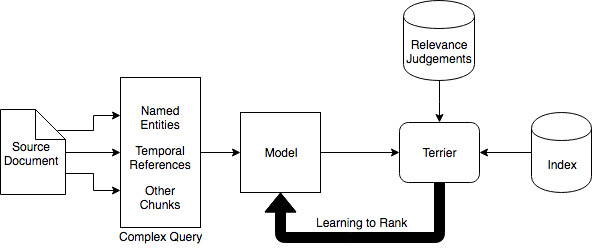
\includegraphics[scale=0.65]{images/5yp-architecture}
\caption{Diagram of Approach for Learning to Rank}
\label{architecture1}
\end{figure}
\begin{figure}[H]
\centering
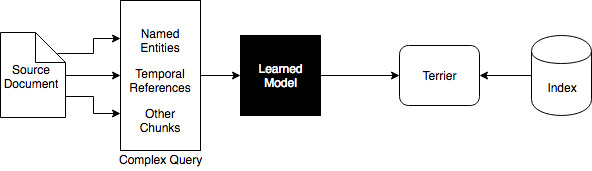
\includegraphics[scale=0.65]{images/5yp-architecture-learned}
\caption{Diagram of Approach with Learned Model for Use During Evaluation}
\label{architecture2}
\end{figure}
Figures~\ref{architecture1} \& \ref{architecture2} provide an overview of the proposed approach.
Figure~\ref{architecture1} demonstrates the learning to rank phase of the project.
As we can see, documents are analysed to form complex queries consisting of named entities, temporal entities. During learning to rank an model will be created and trained based on the features we provide. Terrier will perform retrieval using the model and compare the results to the known results. Depending on the performance the model will be tweaked in order to improve results.
Figure~\ref{architecture2} shows the operation of the retrieval system following the learning of the model. This learned model is used on unseen queries in order to produce relevant results.
In order to use the parts of the complex query, there must be equivalent terms in the index of target documents. This means the analysis steps which extract the named entities and such must be run on all target documents.

\subsection{Evaluation and Experimental Set Up}\label{proposed_approach.evaluation}
Having given an explanation of the proposed approach the implementation of this research will take we now explain how we can evaluate it's effectiveness.

\subsubsection{Hypotheses}
We have formed some hypotheses in response the research questions proposed in Section~\ref{problem_statement}. 
These hypotheses allows us to design and plan efficient experiments for evaluating the effectiveness of our proposed IR system.
Table~\ref{hypotheses.table} gives hypotheses and null hypotheses in direct response to the research questions \textbf{RQ1} and \textbf{RQ2}.

\begin{table}[H]
\centering
\begin{tabular}{|p{2cm}|p{1cm}|p{6cm}|p{6cm}|}
\hline
Relevant Research Question  & Hyp. No.  & Hypothesis & Null Variant     \\ \hline
\multirow{2}{*}{\textbf{RQ1}} & 1 & Inclusion of temporal information in complex queries will improve query performance by promoting those documents which reference these temporal entities in search results. & Including temporal information will have no effect on query performance.\\ \cline{2-4}
& 2 & Adding context, like additional nouns and verbs other than named entities to queries will improve performance when there are many target documents which refer to the included set of named entities. & Including other chunks, like noun phrases will have no effect on query performance. \\ \cline{1-4}
\multirow{2}{*}{\textbf{RQ2}} & 3 & The weighting model created by learning to rank will cause query performance to increase by favouring the features of the queries which perform the best. & Using learning to rank in order to weight the sections of the complex queries will have no effect compared to weighting all query sections equally. \\ \cline{2-4}
& 4 & The complex query generation system will be efficient and the queries will perform better than those queries with only named entities. & We cannot efficiently and effectively extract information from source documents to formulate a complex query consisting of multiple classes of information. \\ \cline{1-4}
\end{tabular}
\caption{Hypotheses and Null Hypotheses in Response to \textbf{RQ1} and \textbf{RQ2}}
\label{hypotheses.table}
\end{table}

These hypotheses will be tested and verified through use of the following measures.

\subsubsection{Effectiveness Measures} \label{evalmeasures}
In order to evaluate the effectiveness of the retrieval system in relation to the above hypotheses we must employ formal measures of comparison.
Information retrieval is usually measured in terms of \textit{precision} and \textit{recall}. \textit{Precision} is the measure of how many of the retrieved documents are relevant, whereas \textit{recall} is a measure of how many of the total number of relevant documents were retrieved.
The most important and ubiquitous measure is \textit{Mean Average Precision} (MAP). 
MAP is commonly used in experiments involving TREC collections as it gives a good objective overview of the performance of a given system and is well understood IR research communities, allowing others to easily interpret results.
\textit{Precision at n} (P@5/10) This measure allows us to measure the precision at the first n documents returned. 
That is, we can see a measure of how effective the system is a retrieving and ranking documents close to the top of the results.
\textit{Mean Reciprocal Rank} (MRR) allows us to measure in a list of ranked results how close the top of the list the first relevant result was. We aim for the first relevant results being high in the ranking of results.

In the L4 Project~\cite{DissertationKelvinFowler} the \textit{All Terms Query} was regarded as too slow to justify its use in an interactive user environment. 
This proposed research is a continued investigation into assisting the sensitivity review process at The National Archives so it is prudent to continue to measure query execution time. We must ensure that query results are returned in a reasonable time and propose to measure query execution time in addition to the standard IR measures above.

\subsubsection{Test Collection}
For evaluation we use a collection of Associated Press articles from the TREC 1 Ad-Hoc task~\footnote{http://trec.nist.gov/}. The documents are a collection of Associated Press articles. These are indeed public domain documents and so are representative of the documents retrieved in the sensitivity review process. There are \textbf{\textit{79919}} documents in the target collection. These are a mixture of news articles. We will be using TREC Topics 51-100 from the TREC-1 Ad-Hoc task along with the supplied relevance judgements for TIPSTER disk 1\&2.

\subsubsection{Using Existing Relevance Judgements} \label{existingrelevance}
% This needs to be as clear as possible
Drawing inspiration from Lee et al~\cite{GeneratingQueriesLee12} we propose to also use the collection of target documents as representative source documents. 
The generation of a test collection is an expensive task which requires many hours of manual work. 
In order to do this we must look specifically at the existing topics and relevance judgements provided for the TREC 1 Ad-Hoc task.
For each topic, the collection of relevant documents can be assumed to be (in some way) all relevant to each other.
Provided the document is analogous in some way to the original query then the information need of ``public domain documents relating to this document'' is fulfilled by the relevant documents according to the qrels for the original topic.
We can form an effective test collection by choosing a number \code{N} of topics. 
For each of these topics we can choose a random relevant document according to the corresponding qrel entry. 
We must then check if the document is representative of the initial topic (as in it is representative of the description in the trec topics file). 
Then this document can be added to the source collection.
The document being used as a source document will be removed from the target collection.

In fact we can make this method even more comprehensive by rotating the document in use as a source document. Given a topic \code{T} and a set of relevant documents \code{D}, we can take every document $ d \in D $. We might assume that if our retrieval system is optimal creating a query from $ d $ would yield $ D \setminus \{d\} $. Thus, we can rotate the proxy source document and attempt to check if this is true. We will then have many more experiment to run, from which to analyse results.

This approach to generating a test collection would not be a suitable substitution in other sensitivity review scenarios. We can use it in this instance since we consider the objective terms and phrases mentioned in a document, which are similar across source and target documents (e.g. named entities, temporal references and noun phrase chunks).
There are some issues with this approach, such as the fact that it has not been specifically noted by archivists to represent the type of document up for review. Further, the target documents are very long in some cases. In the work of Lee et al~\cite{GeneratingQueriesLee12} they merely selected parts of a document to use in a query which meant they could be more specific in choosing appropriately representative sections of text in order to make use of the existing relevance judgements. We propose to use this approach initially however we remain open to generating a manual test collection if the need arises.

\subsubsection{Validation of Results}
Following the evaluation using the test collection generated from target documents we can reuse the target collection from the L4 Project in order to confirm that the new methods offer an improvement upon the much simpler previous approach.
This will validate that our evaluation using existing relevance judgements was effective and can be applied to future sensitivity review tasks.
The test collection from the L4 Project is formed from WikiLeaks documents.
These documents were confirmed by employees at The National Archives to contain sensitivities similar to those that they deal with on a daily basis.
If the proposed system performs well on this test collection, this will be further proof that the approach is valid for real sensitivity review.

\subsection{Summary}
In this section we have outlined the approach we intend to follow in this project. It details the reasoning behind what we plan to do as well as how we intend to evaluate.
We must effectively and efficiently extract relevant data from source documents. 
This data can be composed into a complex query to run in Terrier against the collection of target documents. 
We can use learning to rank to automatically weight the different sections of the query in order to improve performance on unseen documents.
We can then evaluate this approach using existing documents collections as a test collection, in order to demonstrate the effectiveness of the new system.
The next section gives a more detailed view of how we intend to implement sections of this approach. 

%%%%%%%%%%%%%%%%%%%%%%%%%%%%%   WORK PLAN  %%%%%%%%%%%%%%%%%%%%%%%%%%%%%%%%%%%%%
\section{Work Plan} \label{work_plan}
With the proposed approach detailed in the previous section we can describe some implementation details of this proposed approach and define some milestones of completion.
% With the above proposed approach in mind we can set some definitive milestones for this research project.

% With the proposed approach laid out above in Section~\ref{proposed_approach} we can now give a definitive description of the work that will need to be done in order to complete this research. This section will give an overview of the tasks that must be completed and will end with a Gantt Chart defining time scales for each section.

% Theres gotta be an indexing phase, applied to both the source and target collections
% This indexing phase is going to have various steps, each of which you can describe in some detail.
% Then, depending on if it's source or target documents you actually have to something concrete with the info you extract.
% For source you'll be extracting and saving the individual bits in order to generate queries at a later date (might be a nice idea to allow different query formulations from one indexing pass)
% For target you need to add the terms to various (posting lists?????)
% Next is actual query generation, this isnt a textual thing to you can describe how you plan to pass the subquery components to terrier programatically.
% Then theres the actual retrieval, as in plumbing it all together to let terrier do it's thing.
% Then there's learning to rank where we let terrier figure out how to weight the different features (whatever these features might be, need to be clear about that)
% Evaluation next, create the test collection
% Do the evaluation using trec_eval in built into terrier
% Analyse the results
% Write up the dissy

% Theres very clear steps here, how do you go about seperating the ``proposed apporach'' to the work plan. Like where do we do the comparison of heideltime and sutime.
% Need to somehow effectively describe what a feature is....
\subsection{Query Component Extraction}
In order to formulate our complex queries as described in Section~\ref{proposedapproach.complexquery}, we must create a system which can read in a source document and return a collection of the complex query components. 
In order to extract the Named Entities we can continue to use StanfordNLP in a similar way to the L4 Project, with some slight adjustments.
This has been prototyped and we have successfully extracted n-gram named entities in order to retain multi word relationships.

We propose to use Heideltime for the extraction of temporal entities.
This works well with no major alterations and the times can be extracted programatically.
A particular challenge while indexing the target collection may be the identification of document creation times.
Confusingly, these exist as part of the Doc Id of each document and so some parser will need to be implemented to extract the dates from here.
This should be relatively simple.
It remains only to convert the Heideltime output into our desired format for storing temporal information.
Initially, at least, we wish to store temporal entities as a string so they can be directly compared to times mentioned in target documents during retrieval.
Instead we propose simply to use YYYYMMDD format.

We also wish to exact other chunks from text in order to form queries.
This could be noun phrases or verb phrases or other constructions.
In order to do this we can again use the Stanford NLP toolkit.
It includes the Stanford Parser which annotates sentences with parts of speech tags.
We can identify different constructions using these parts of speech tags.

Each of these extraction steps will have to be implemented in a way which not only interacts well with indexing but can also be used in a standalone sense to create queries from documents.


\subsection{Complex Queries}
With these query components created we can now explicitly form our complex query, using the complex query features provided by Terrier v5. 
The inclusion of complex query features in Terrier is very new and there is little example code or documentation.
This will therefore require much experimentation and investigation.
It may be required to implement some  custom extensions to the complex query system in Terrier in order to achieve the exact custom query formulation we wish to create.
For example, we may have to make new custom sizes of unordered windows. 
This query will not be provided to Terrier as merely text, but rather programmatically. 
Initially these queries will take a simple form of the various query components discussed above.
However, following successful evaluation of these query formulations we will begin a second phase which investigates more complex query formulations and methods.

Some combination of the extractors discussed above will be used in a class which receives a full document and outputs a complex query formulation.
This complex query will be modelled by a class in Java.

\subsection{Learning to Rank}
Upon the creation of complex queries and completion of target collection indexing, we will have a working initial retrieval system which can be evaluated in order to obtain baseline results.
In order to improve the performance and to obtain data relating to the performance of individual query sections we now wish to apply learning to rank.
Terrier provides learning to rank functionality as standard.
We will be using the JForests\footnote{http://code.google.com/p/jforests/} implementation of LambdaMART~\cite{wu2008ranking}.
Depending on the implementation of the above steps, we will produce a set of features, both query dependent and independent.
These features will be applied in learning to rank in different combinations.
The evaluation process must continue throughout this experimentation with feature combinations in order to discover the best configuration.
Specifically our set of features must include features which directly correlate to the use of section of a query, so that we may measure it's effectiveness and apply a ``weight'' to it.
We will not manually apply weights, instead the L2R process will achieve this for us.

Learning to rank relies on a sampling step, both during learning and application of the learned model~\cite{macdonald2013whens}.
Generally, a simpler retrieval approach such as BM25 is used at this stage to achieve high recall.
The reranking step then uses the complex query with the defined features to reorder the results.
For our approach, this initial sampling step will also require some investigation.
Although we may use a more basic retrieval model, a query is still required.
This may just be all the terms in the document with stopwords removed, although this will be slow.

The existing relevance judgements in the test collection can be used to train the model. 
Following the creation of more complex query formulations we will once again use learning to rank to learn a model for retrieval based on features from these complex queries.

The completion of the learning to rank phase effectively completes the proposed approach, with only evaluation left to continue.

\subsection{Evaluation}
We now describe the plan for the evaluation stages of the project.

\subsubsection{Formulate Test Collection}
As early as is feasible we should seek to formulate a reasonably large test collection using the approach described in Section~\ref{proposed_approach.evaluation}.
We must create an automated system that can use the relevance judgement files to automatically perform evaluation in a rotation using all the relevant documents for that topic as source documents, one at a time.
We can use the evaluation scripts included with Terrier to facilitate this, although some additional code will be required.

\subsubsection{Evaluation of System}
With the test collection formed, we should design experiments in direct response to the hypotheses defined in Section~\ref{proposed_approach.evaluation}.
Using the automated evaluation tool with the test collection described above, we must change one aspect of the system at a time in order to effectively evaluate.
These experiments directly correspond to the hypotheses of Table~\ref{hypotheses.table} and are ordered from the simplest to the most complex. 
Table~\ref{proposed_experiments} shows these hypotheses and also make clear which part of the system they intend to evaluate.
In order to test the effectiveness of each individual query component we will perform experiments using the initial extracted information in different combinations.
We will then evaluate the effectiveness of learning to rank with different features.
Retrieval performance will be a combination of measures as defined in Section~\ref{proposed_approach.evaluation}, including query processing time.
The first four experiments in Table~\ref{proposed_experiments} can be performed as soon as query component extraction and complex query generation is complete. 
This will allow us to perform queries using different combinations of components. 
There will be no learned model at this stage applying weights to features and this will be evaluated separately.
Beginning experiments early has the advantages of inspiring ideas for continuing work as we move through the project.
It also allows for the identification of bugs and problems at an early stage.

\begin{table}[H]
\centering
\begin{tabular}{|p{2cm}|p{2cm}|p{6cm}|p{4cm}|}
\hline
Relevant Research Question & Relevant Hypothesis & Experiment & Target Component \\ \hline
\multirow{4}{*}{\textbf{RQ1}} & \multirow{2}{*}{1} & Retrieval performance with only improved named entity extraction & Named Entity Extraction \\ \cline{3-4}
& & Retrieval Performance with Named Entities and Temporal Entities & Temporal Entity Extraction \\ \cline{2-4}
& \multirow{2}{*}{2} &  Retrieval Performance with Named Entities and Other Chunks & Chunk Extraction for Context \\ \cline{3-4}
& & Retrieval Performance with Named Entities, Temporal Entities and Other Chunks & All Query Section Extraction Methods \\ \cline {1-4}
\multirow{3}{*}{\textbf{RQ2}} & \multirow{2}{*}{3} & Retrieval Performance prior to applying a learned model & Learning to Rank \\ \cline{3-4}
& & Retrieval performance following the application of a learned model from learning to rank with different feature combinations & Learning to Rank \\ \cline{2-4}
& 4 & Retrieval performance combining the proven best concepts from the above experiments & Entire Retrieval System \\ \cline{1-4}
\end{tabular}
\caption{Proposed Experiments and their Purpose}
\label{proposed_experiments}
\end{table}

\subsection{Further Work}
This work plan is flexible and allows the ability to add other items as we proceed. 
Once all of the above has been completed and evaluated we can look forwards to improving the query generation stage even more. 
Some potential avenues are query expansion through knowledge base linking or allowing more generality in temporal comparisons. 
We may also formulate and additional test collection in order to perform additional evaluation to more concretely rate the performance of our system.

\subsection{Time Frames}
The Gantt chart in Table~\ref{gantt} displays the proposed time frames for the above planned work. This Gantt chart is merely an indication of the time that may be spent on each item. Work will be completed as quickly as possible in order to try to allow for more experimentation with more complex ideas. The gap in implementation of complex queries and learning to rank demonstrates a pause for evaluation and then a second phase investigating more complex query formulations and learned models based on these.
% A table with rows containing a pbox of 0.17 textwidth, followed by 20 pboxes
% of 0.01 textwidth. Although this sums to just 0.37 textwidth, there are a
% lot of intercolumn gaps to consider. The 0.17 and 0.01 were fiddled by hand
% to fit this particular example.
\begin{table}
\noindent\begin{tabular}{p{0.17\textwidth}
!{\vrule width 0.4mm}p{0.01\textwidth}*{3}{|p{0.01\textwidth}}
!{\vrule width 0.4mm}p{0.01\textwidth}*{3}{|p{0.01\textwidth}}
!{\vrule width 0.4mm}p{0.01\textwidth}*{3}{|p{0.01\textwidth}}
!{\vrule width 0.4mm}p{0.01\textwidth}*{3}{|p{0.01\textwidth}}
!{\vrule width 0.4mm}p{0.01\textwidth}*{3}{|p{0.01\textwidth}}
|}
% The top line
\textbf{Gantt chart} & \multicolumn{4}{c!{\vrule width 0.4mm}}{December} 
& \multicolumn{4}{c!{\vrule width 0.4mm}}{January}
& \multicolumn{4}{c!{\vrule width 0.4mm}}{February} 
& \multicolumn{4}{c!{\vrule width 0.4mm}}{March} 
& \multicolumn{4}{c|}{April} \\
% The second line, with its five years of four quarters
%\rpt[5]{& 1 & 2 & 3 & 4} \\
\hline
% using the on macro to fill in twenty cells as `on'
Query \mbox{Component} \mbox{Extraction}        \on[6] \off[14] \\
\hline
Complex Query Formulations   \off[4] \on[4] \off[4] \on[2] \off[6] \\
\hline
Learning to Rank   \off[4] \on[4] \off[4] \on[2] \off[6] \\
\hline
Evaluation using Test Collection    \off[3] \on[17]  \\
\hline
% using the on macro followed by the off macro
Write-Up     \off[16] \on[4]\\
\hline
\end{tabular}
\caption{Gantt Chart of Proposed Work Plan}
\label{gantt}
\end{table}

%%%%%%%%%%%%%%%%%%%%%%%%%%%%%%%%%%%%%%%%%%%%%%%%%%%%%%%%%%%%%%%%%%%
% it is fine to change the bibliography style if you want
\bibliographystyle{plain}
\bibliography{mprop}
\end{document}
